\documentclass[11pt]{article}
\usepackage[letterpaper,margin=1in,top=0.9in,bottom=0.9in]{geometry}
\usepackage{amsmath,amssymb,amsthm,mathtools}
\usepackage{tikz}
\usetikzlibrary{arrows.meta,positioning,calc}
\usepackage{forest}
\usepackage{array}
\usepackage{fancyhdr}
\usepackage{enumitem}
\usepackage{tabularx}
\usepackage{multicol}

\setlength{\parindent}{0pt}
\setlength{\parskip}{4pt}

% ---- course notation macros ----
\newcommand{\N}{\mathbb{N}}
\newcommand{\Z}{\mathbb{Z}}
\newcommand{\Q}{\mathbb{Q}}
\newcommand{\R}{\mathbb{R}}
\newcommand{\Cx}{\mathbb{C}}
\newcommand{\nuc}{\nu} % cardinality
\newcommand{\Fnc}[2]{\mathit{Fnc}(#1,#2)}
\newcommand{\Rflx}[1]{\mathit{Rflx}(#1)}
\newcommand{\Sym}[1]{\mathit{Sym}(#1)}
\newcommand{\Trns}[1]{\mathit{Trns}(#1)}
\newcommand{\AntSym}[1]{\mathit{AntSym}(#1)}
\newcommand{\Eqv}[1]{\mathit{Eqv}(#1)}
\newcommand{\PO}[1]{\mathit{PO}(#1)}
\newcommand{\EqvCl}[2]{\mathit{EqvCl}(#1,#2)}
\newcommand{\HsDgrm}[1]{\mathit{HsDgrm}(#1)}
\newcommand{\Tlg}[1]{\mathit{Tlg}(#1)}
\newcommand{\Cdn}[1]{\mathit{Cdn}(#1)}
\newcommand{\Cng}[1]{\mathit{Cng}(#1)}
\newcommand{\TT}[1]{\mathit{TT}(#1)}
\newcommand{\barr}{\rule{0.98\linewidth}{0.5pt}}
\newcommand{\shortbar}[1]{\rule{#1}{0.5pt}}

% single-bar inference: premise over an auto-width rule over conclusion (matches the
% exam pipeline's \INFBAR -- bar spans exactly max(premise,conclusion), never a guessed width)
% \Inf{premise}{conclusion} ; \Infw{premise}{conclusion}{witness} puts a <var<-expr> chevron to the right
\newcommand{\Inf}[2]{\begin{tabular}[c]{@{}c@{}}$#1$\\\hline$#2$\end{tabular}}
\newcommand{\Infw}[3]{\Inf{#1}{#2}\ \ $\langle #3 \rangle$}
% \Subs stacks several var<-expr assignments inside one tall chevron pair
\newcommand{\Subs}[1]{\left\langle\begin{tabular}[c]{@{}l@{}}#1\end{tabular}\right\rangle}

% boxed piece label, top-left of a piece (matches \PLBL)
\newcommand{\PL}[1]{\noindent\fbox{\footnotesize #1}\par\vspace{2pt}}

% BC / RcS / SPf / EPf induction-proof scaffolding (per course's confirmed template)
\newenvironment{spf}{\par\noindent\textbf{SPf}\par\vspace{2pt}}{\par\vspace{2pt}\noindent\textbf{EPf}\par}
\newcommand{\bclabel}{\textbf{BC}\par}
\newcommand{\rcslabel}{\textbf{RcS}\par}

% one small binary-connective truth table + words, for 2(11)
\newcommand{\conntable}[6]{%
  \begin{minipage}[t]{0.24\linewidth}
  \centering \footnotesize $c_{#1}$\\[2pt]
  \begin{tabular}{cc|c}
  $p$&$q$&$c_{#1}$\\\hline
  0&0&#2\\0&1&#3\\1&0&#4\\1&1&#5
  \end{tabular}\\[3pt]
  \footnotesize #6
  \end{minipage}%
}

% folio box, lower right corner of a work sheet
\newcommand{\folio}[1]{%
  \begin{tikzpicture}[remember picture,overlay]
    \node[anchor=south east,xshift=-0.6in,yshift=0.5in,draw,minimum width=0.45in,minimum height=0.16in,inner sep=1pt] at (current page.south east) {\small #1};
  \end{tikzpicture}%
}

\pagestyle{fancy}
\fancyhf{}
\renewcommand{\headrulewidth}{0pt}
\renewcommand{\footrulewidth}{0pt}
\fancyhead[L]{\footnotesize Due by2359 hours on 20260818}
\fancyhead[R]{\footnotesize 163 Problem Set}
\fancyfoot[L]{\footnotesize You are free to talk to anyone}
\fancyfoot[R]{\footnotesize\thepage}

% blank work-sheet page style: no header, folio box lower right instead of normal footer
\fancypagestyle{worksheet}{%
  \fancyhf{}
  \renewcommand{\headrulewidth}{0pt}
  \renewcommand{\footrulewidth}{0pt}
}

\usepackage{pdfpages}

\begin{document}

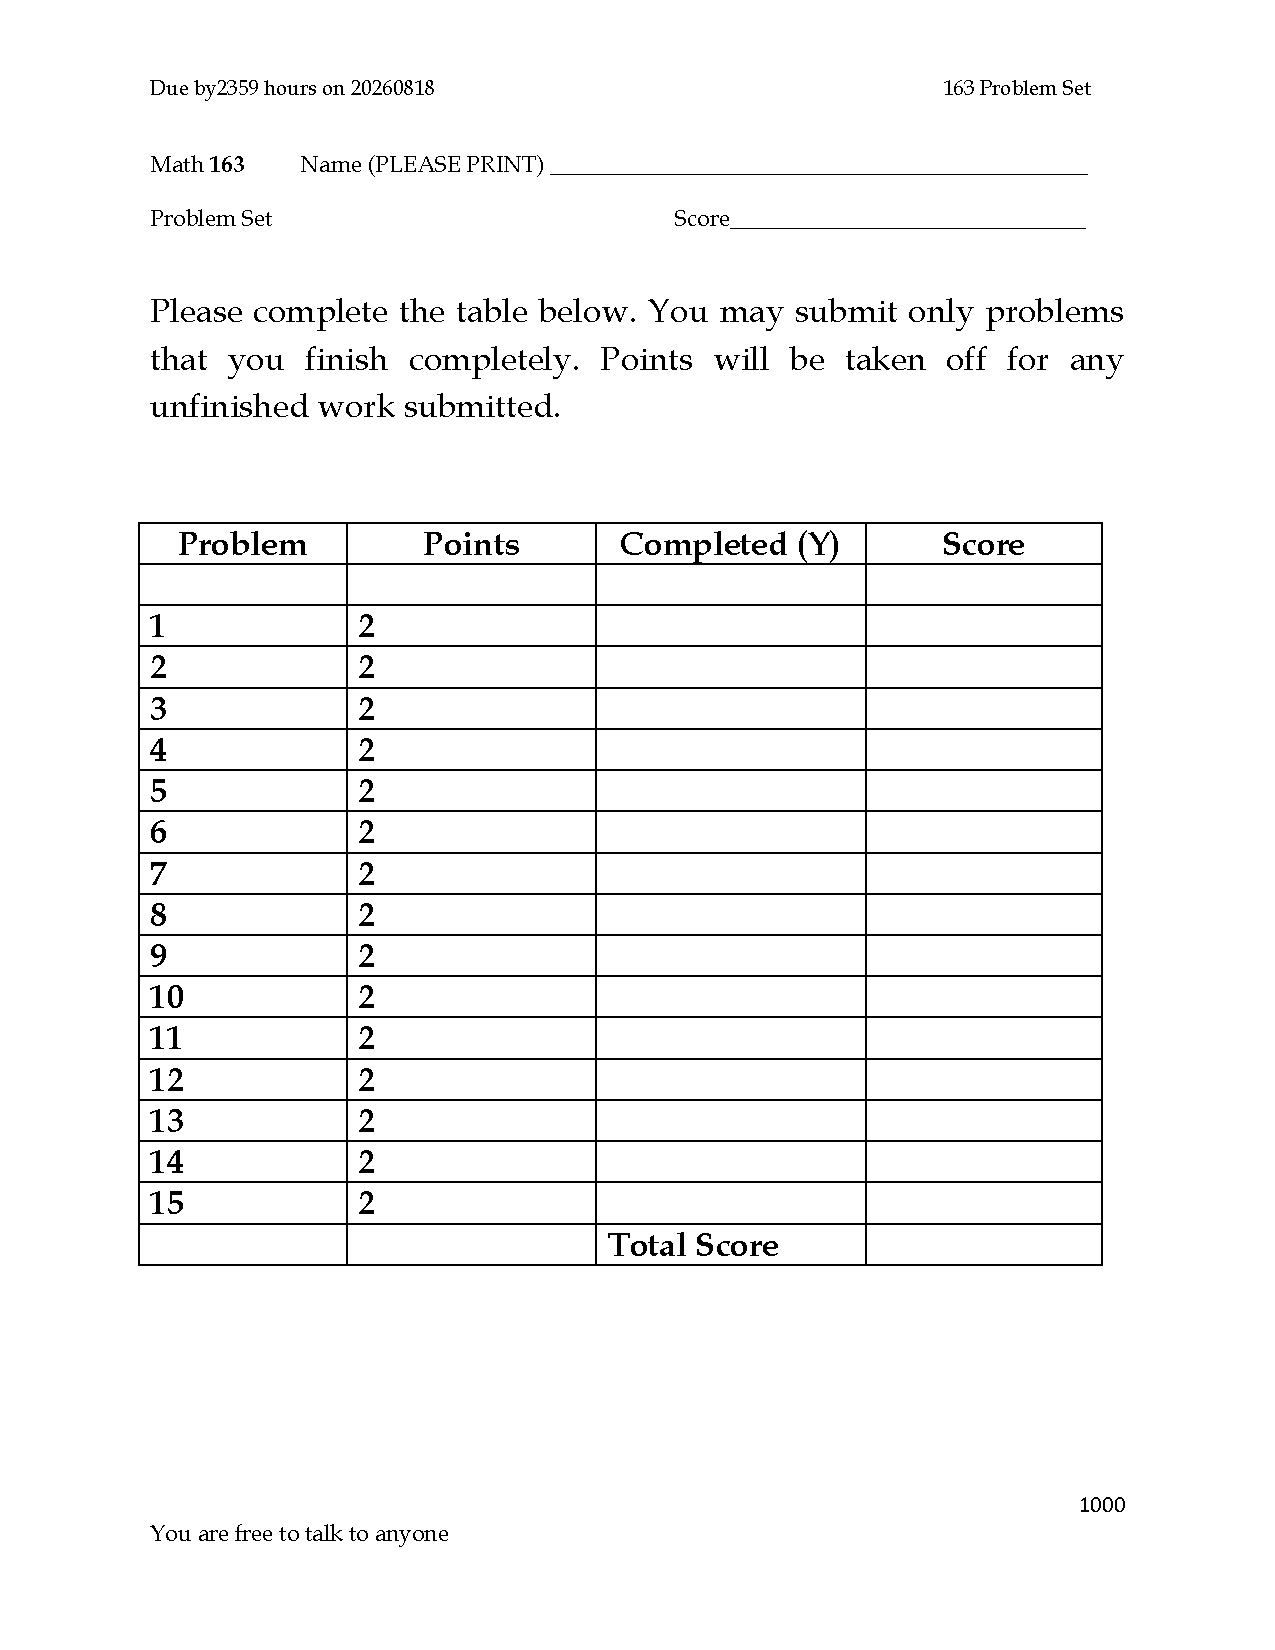
\includepdf[pages=1-3]{../163ProblemSet.pdf}

%=================================================================
% 2(1)  folio 1003
%=================================================================
\fancyfoot[R]{\footnotesize 1003}
\noindent\textbf{2 (1)} \quad Find (and recall) a recursive definition for each of the functions below

\begin{center}
$\varphi \coloneqq n \mapsto n! : \N \longrightarrow \N$ \quad and \quad
$\psi \coloneqq n \mapsto 2^n : \N \longrightarrow \N$
\end{center}

\noindent Prove by induction that: $\forall n \in \N \ \ \varphi(n+4) \geq \psi(n+4)$

\vspace{10pt}
\textbf{D} \quad $\varphi$:

\bclabel
\hspace{1em}$\varphi(0)\coloneqq1$

\rcslabel
\hspace{1em}$\forall n\in\N\ \ \varphi(n+1)\coloneqq(n+1)\varphi(n)$

\textbf{D} \quad $\psi$:

\bclabel
\hspace{1em}$\psi(0)\coloneqq1$

\rcslabel
\hspace{1em}$\forall n\in\N\ \ \psi(n+1)\coloneqq2\,\psi(n)$

\newpage
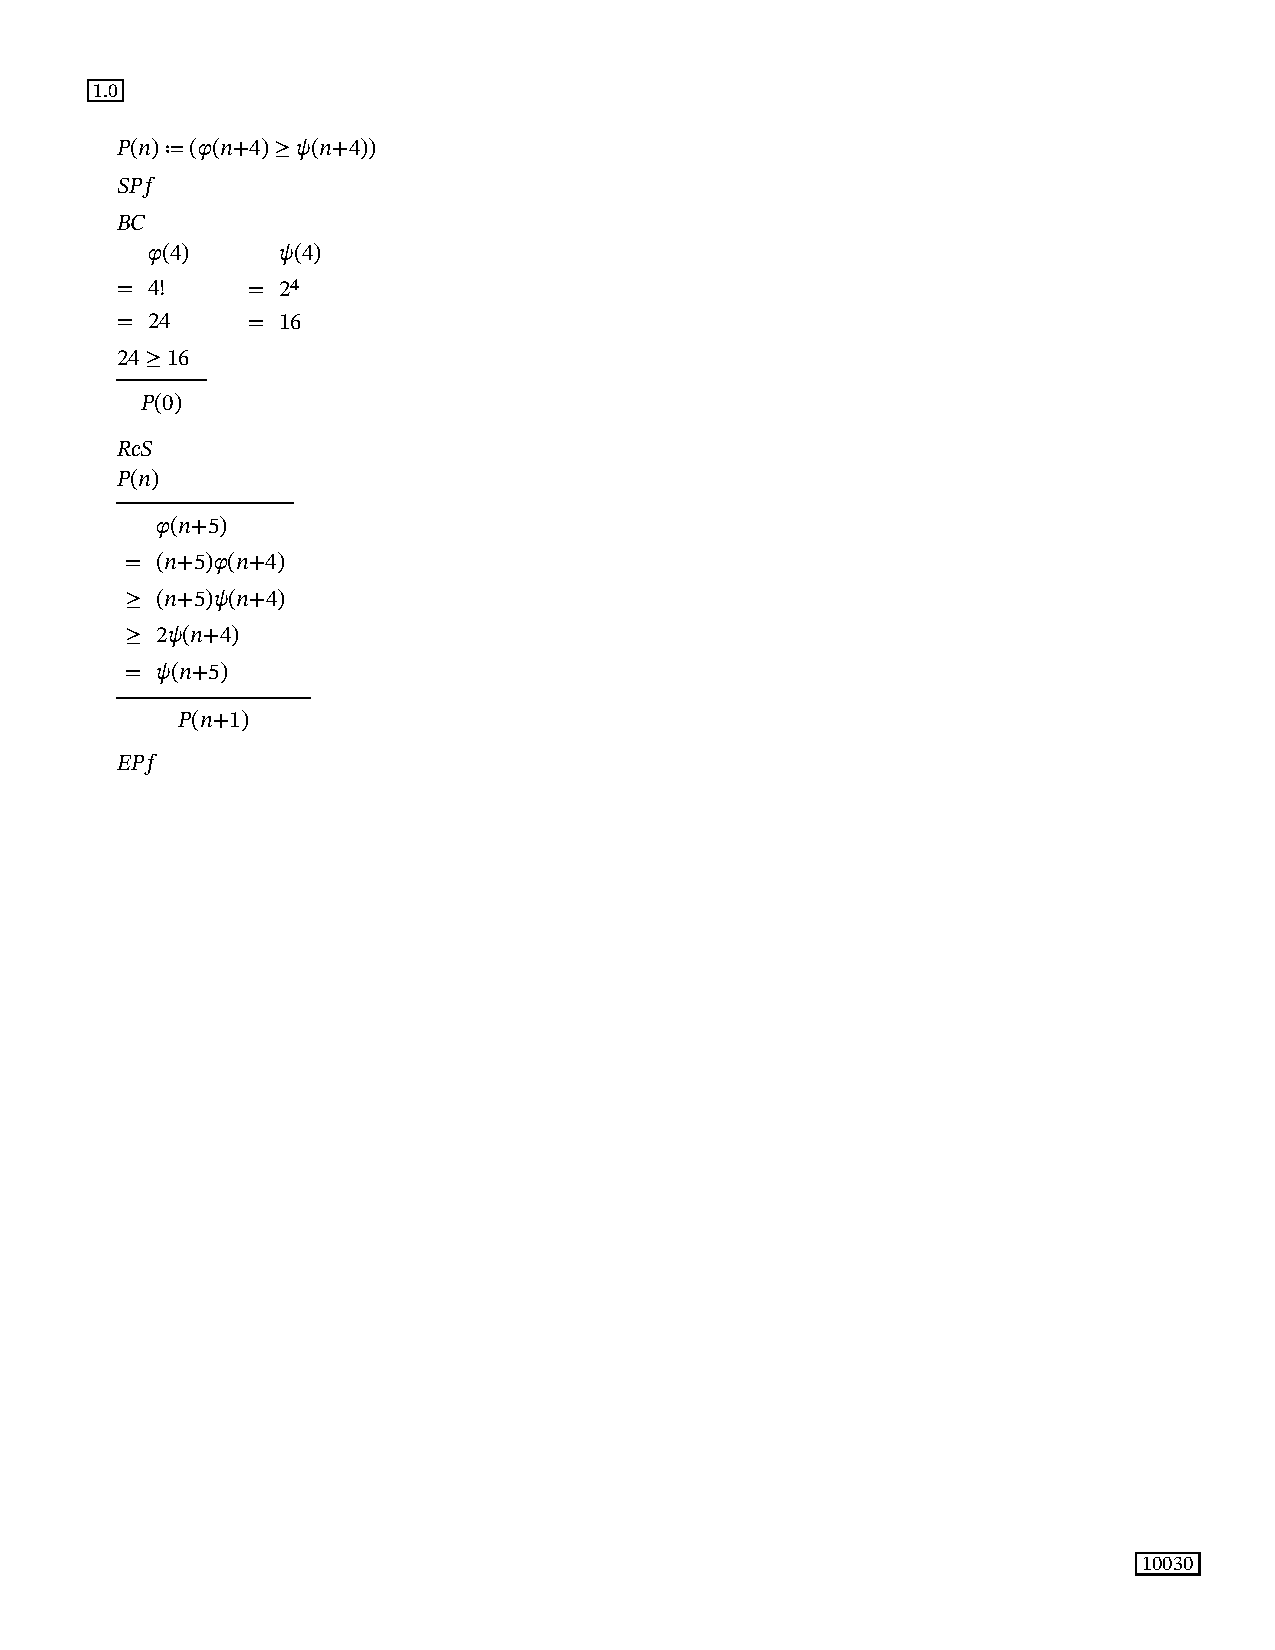
\includepdf[pages=1]{worksheets.pdf}
%=================================================================
% 2(2)  folio 1005
%=================================================================
\newpage
\fancyfoot[R]{\footnotesize 1005}
\noindent\textbf{2 (2)} \quad Starting with sets $A,B,C,D,E$ and $F$ with $a\coloneqq\nuc(A)$, $b\coloneqq\nuc(B)$, $c\coloneqq\nuc(C)$, $d\coloneqq\nuc(D)$, $e\coloneqq\nuc(E)$ and $f\coloneqq\nuc(F)$, use as many of the operations in the list below as many times as you wish:
$$\left\{\ (\ )^c,\ \cup,\ \cap,\ \backslash,\ \prod{},\ \coprod{},\ \Fnc{A}{B},\ (\ ),\ \sim\ \right\}$$
(i) to construct a set $S$ whose cardinality appears below, and
$$\nuc(S) = a+b-c\times d \div e \wedge f$$
(ii) to construct word-problems whose solutions require counting the number of elements of the sets you constructed in (i). Note that the numbers are such that $\nuc(S)\in\N$. Draw a formation-tree for the expression on the facing side. Draw a formation-tree for the expression that you have constructed. Prove that the cardinality of the set that you have constructed equals the given expression. Write the word problem step by step respecting the formation-tree of the expression that you have constructed.

\vspace{6pt}
$a=5,\ b=4,\ c=2,\ d=3,\ e=2,\ f=1$.

$G\coloneqq\Fnc{F}{E}$;\quad $P\coloneqq C\times D$;\quad $W$: eq.\ rel.\ on $P$, classes of size $\nuc(G)$;\quad $Q\coloneqq P/W$;\quad $S\coloneqq(A\sqcup B)\setminus Q$, $Q\subseteq A\sqcup B$.


\newpage
\thispagestyle{worksheet}
\folio{10050}
\PL{2.0}

\begin{center}
\begin{forest}
for tree={edge={-},l sep=18pt,s sep=14pt,anchor=center,inner sep=2pt}
[$-$
  [$+$ [$a$] [$b$]]
  [$\div$ [$\times$ [$c$] [$d$]] [$\wedge$ [$e$] [$f$]]]
]
\end{forest}
\end{center}

\vspace{6pt}
\PL{2.1}

\begin{center}
\begin{forest}
for tree={edge={-},l sep=18pt,s sep=14pt,anchor=center,inner sep=2pt}
[$\setminus$
  [$\sqcup$ [$A$] [$B$]]
  [$/W$ [$\times$ [$C$] [$D$]]]
]
\end{forest}
\end{center}

\newpage
\thispagestyle{worksheet}
\folio{10051}
\PL{2.2}

\hspace{1em}\Inf{Q\subseteq A\sqcup B}{(A\sqcup B) = \big((A\sqcup B)\setminus Q\big)\cup Q}

\hspace{1em}$\nuc(A\sqcup B)=\nuc(A)+\nuc(B)=a+b=\nuc(S)+\nuc(Q)$

\hspace{1em}$\nuc(P)=\nuc(C\times D)=\nuc(C)\times\nuc(D)=c\times d$

\hspace{1em}$\nuc(\Fnc{F}{E})=\nuc(E)^{\nuc(F)}=e\wedge f=\nuc(G)$

\hspace{1em}$\nuc(Q)=\nuc(P/W)=\nuc(P)\div\nuc(G)=(c\times d)\div(e\wedge f)$

\hspace{1em}$\nuc(S)=\nuc(A\sqcup B)-\nuc(Q)=(a+b)-\big((c\times d)\div(e\wedge f)\big)=6$ \hfill$\blacksquare$

\vspace{10pt}
\PL{2.3}

$C$: $2$ breads. $D$: $3$ fillings. $\to\nuc(C\times D)=6$ sandwiches.

$E$: $2$ sizes. $F$: $1$ cup. $\to\nuc(\Fnc{F}{E})=2$ size-assignments.

Group the $6$ sandwiches into groups of $2$. $\to\nuc(Q)=3$ groups.

$A$: $5$ people, table $1$. $B$: $4$ people, table $2$. $\to\nuc(A\sqcup B)=9$.

One person leaves per group ($3$ groups). $\to\nuc(S)=9-3=6$ people remain.

%=================================================================
% 2(3)  folio 1007
%=================================================================
\newpage
\fancyfoot[R]{\footnotesize 1007}
\noindent\textbf{2 (3)} \quad Define a relation on $\N$ as follows:
$$\forall x,y\in\N\quad (xRy)\coloneqq(x\mid y)$$
Prove that: $\PO{R,\N}$

\vspace{4pt}
Draw the Hasse Diagram for the $\{J_k \mid k\in 1..8\}$ under divisibility ordering $\mid$, that is:
$$\HsDgrm{\{J_k\mid k\in 1..8\},\mid}$$

\vspace{6pt}
$J=00499317 \implies \{J_k\mid k\in1..8\}=\{0,1,3,4,7,9\}$.


\begin{center}
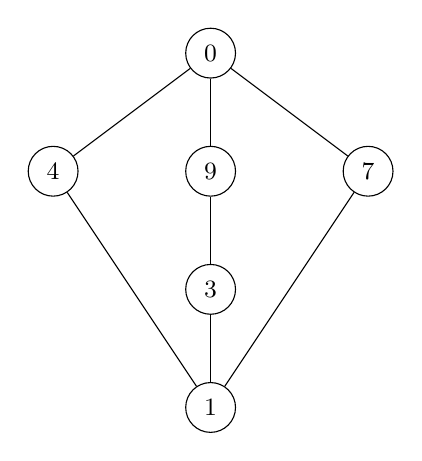
\begin{tikzpicture}[every node/.style={draw,circle,minimum size=18pt,inner sep=0pt,font=\small}]
\node (n0) at (0,4.5) {$0$};
\node (n4) at (-2,3) {$4$};
\node (n9) at (0,3) {$9$};
\node (n7) at (2,3) {$7$};
\node (n3) at (0,1.5) {$3$};
\node (n1) at (0,0) {$1$};
\draw (n1) -- (n3);
\draw (n1) -- (n4);
\draw (n1) -- (n7);
\draw (n3) -- (n9);
\draw (n4) -- (n0);
\draw (n7) -- (n0);
\draw (n9) -- (n0);
\end{tikzpicture}
\end{center}

\newpage
\includepdf[pages=2-3]{worksheets.pdf}
%=================================================================
% 2(4)  folio 1009
%=================================================================
\newpage
\fancyfoot[R]{\footnotesize 1009}
\noindent\textbf{2 (4)} \quad Define a relation on $\Z$ as follows:
$$\forall x,y\in\Z\quad (xRy)\coloneqq(x^2=y^2)$$
Prove that: $\Eqv{R,\Z}$ and find the equivalence classes.

\vspace{6pt}
$\Z/R = \big\{\{0\}\big\} \cup \big\{\{-n,n\} \mid n\in\N,\, n\geq 1\big\}$

\newpage
\includepdf[pages=4-5]{worksheets.pdf}
%=================================================================
% 2(5)  folio 1011
%=================================================================
\newpage
\fancyfoot[R]{\footnotesize 1011}
\noindent\textbf{2 (5)} \quad Define a relation on $\N\times\N$ as follows:
$$\forall (a,b),(c,d)\in\N\times\N \quad \big((a,b)R(c,d)\big)\coloneqq\big(a+b=c+d\big)$$
Prove that: $\Eqv{R,\N\times\N}$ and find the equivalence classes.

\vspace{6pt}
$(\N\times\N)/R = \{\{(0,k),(1,k-1),\dots,(k,0)\} \mid k\in\N\}$

\newpage
\includepdf[pages=6-7]{worksheets.pdf}
%=================================================================
% 2(6)  folio 1013
%=================================================================
\newpage
\fancyfoot[R]{\footnotesize 1013}
\noindent\textbf{2 (6)} \quad Define a relation on $\N\times\N$ as follows:
$$\forall (a,b),(c,d)\in\N\times\N \quad \big((a,b)R(c,d)\big)\coloneqq\big(a^2+b^2=c^2+d^2\big)$$
Prove that: $\Eqv{R,\N\times\N}$ and find the equivalence classes.

\vspace{6pt}
$(\N\times\N)/R = \big\{\{(x,y)\in\N\times\N\mid x^2+y^2=n\}\ \big|\ n\in\N,\ \exists(x,y)\,(n=x^2+y^2)\big\}$

\newpage
\includepdf[pages=8-9]{worksheets.pdf}
%=================================================================
% 2(7)  folio 1015
%=================================================================
\newpage
\fancyfoot[R]{\footnotesize 1015}
\noindent\textbf{2 (7)} \quad Find a formula for the Fibonacci Numbers by solving the recurrence below. The Fibonacci numbers are defined recursively as follows:
$$\begin{cases}\rho(0)\coloneqq 0\\ \rho(1)\coloneqq 1\\ \forall n\in\N \quad \rho(n+2)-\rho(n+1)-\rho(n)=0\end{cases}$$

\vspace{6pt}
$c_2=1,\ c_1=-1,\ c_0=-1,\ R_0=0,\ R_1=1,\quad r\coloneqq\dfrac{-c_1}{2c_2}=\dfrac12,\quad s\coloneqq\dfrac{\sqrt{c_1^2-4c_2c_0}}{2c_2}=\dfrac{\sqrt5}{2}$

Formula $11$ (Induction and Recursion Notes p.\,26).
$$\rho(n) = \frac{1}{\sqrt5}\left(\left(\frac{1+\sqrt5}{2}\right)^{\!n} - \left(\frac{1-\sqrt5}{2}\right)^{\!n}\right)$$

\newpage
\includepdf[pages=10]{worksheets.pdf}
%=================================================================
% 2(8)  folio 1017
%=================================================================
\newpage
\fancyfoot[R]{\footnotesize 1017}
\noindent\textbf{2 (8)} \quad Prove by induction that:
$$S(2,n)\coloneqq\sum_{k=0}^n k^2 \ =\ \frac{n(n+1)(2n+1)}{6}$$

\vspace{6pt}
\newpage
\includepdf[pages=11]{worksheets.pdf}
%=================================================================
% 2(9)  folio 1019
%=================================================================
\newpage
\fancyfoot[R]{\footnotesize 1019}
\noindent\textbf{2 (9)} \quad Use the method of differences shown in class to find a recursive definition of:
$$S(3,n)\coloneqq\sum_{k=0}^n k^3$$
Prove by induction that:
$$S(3,n)\coloneqq\sum_{k=0}^n k^3 = \big(S(1,n)\big)^2$$

\vspace{6pt}
\bclabel
\hspace{1em}$S(3,0)\coloneqq0$

\rcslabel
\hspace{1em}$\forall n\in\N\ \ S(3,n+1)\coloneqq S(3,n)+(n+1)^3$

$S(1,n)=\dfrac{n(n+1)}{2}$.

\newpage
\includepdf[pages=12]{worksheets.pdf}
%=================================================================
% 2(10)  folio 1021
%=================================================================
\newpage
\fancyfoot[R]{\footnotesize 1021}
\noindent\textbf{2 (10)} \quad Find (and recall) a recursive definition for each of the functions below

\begin{center}
$\beta \coloneqq n \mapsto n! : \N \longrightarrow \N$ \quad and \quad
$\gamma \coloneqq n \mapsto n^n : \N \longrightarrow \N$
\end{center}

\noindent Prove by induction that: $\forall n \in \N \ \ \gamma(n) \geq \beta(n)$

\vspace{10pt}
\textbf{D} \quad $\beta$:

\bclabel
\hspace{1em}$\beta(0)\coloneqq1$

\rcslabel
\hspace{1em}$\forall n\in\N\ \ \beta(n+1)\coloneqq(n+1)\beta(n)$

\textbf{D} \quad $\mathrm{exp}\coloneqq(a,n)\mapsto a^n$:

\bclabel
\hspace{1em}$\mathrm{exp}(a,0)\coloneqq1$

\rcslabel
\hspace{1em}$\forall n\in\N\ \ \mathrm{exp}(a,n+1)\coloneqq a\cdot\mathrm{exp}(a,n)$

\hspace{1em}$\gamma(n)\coloneqq\mathrm{exp}(n,n)$

\vspace{4pt}
\newpage
\includepdf[pages=13]{worksheets.pdf}
%=================================================================
% 2(11)  folio 1023
%=================================================================
\newpage
\fancyfoot[R]{\footnotesize 1023}
\noindent\textbf{2 (11)} \quad Find truth-tables for each of 16 binary connectives $\left(c_k \mid k\in1..(16)\right)$ for Boolean Logic and express each formula $pc_kq$ in words.

\vspace{6pt}
Rows $(p,q)=(0,0),(0,1),(1,0),(1,1)$.

\newpage
\thispagestyle{worksheet}
\folio{10230}
\PL{11.0}

\vspace{4pt}
\conntable{1}{0}{0}{0}{0}{always false}
\conntable{2}{0}{0}{0}{1}{$p$ and $q$}
\conntable{3}{0}{0}{1}{0}{$p$ and not $q$}
\conntable{4}{0}{0}{1}{1}{$p$}

\vspace{14pt}
\conntable{5}{0}{1}{0}{0}{$q$ and not $p$}
\conntable{6}{0}{1}{0}{1}{$q$}
\conntable{7}{0}{1}{1}{0}{exactly one of $p,q$}
\conntable{8}{0}{1}{1}{1}{$p$ or $q$}

\vspace{14pt}
\conntable{9}{1}{0}{0}{0}{neither $p$ nor $q$}
\conntable{10}{1}{0}{0}{1}{$p$ iff $q$}
\conntable{11}{1}{0}{1}{0}{not $q$}
\conntable{12}{1}{0}{1}{1}{if $q$ then $p$}

\newpage
\thispagestyle{worksheet}
\folio{10231}
\PL{11.1}

\vspace{4pt}
\conntable{13}{1}{1}{0}{0}{not $p$}
\conntable{14}{1}{1}{0}{1}{if $p$ then $q$}
\conntable{15}{1}{1}{1}{0}{not both $p$ and $q$}
\conntable{16}{1}{1}{1}{1}{always true}

%=================================================================
% 2(12)  folio 1024
%=================================================================
\newpage
\fancyfoot[R]{\footnotesize 1024}
\noindent\textbf{2 (12)} \quad Define that set of truth-values $\ TV\coloneqq\{-1,0,1\}$

(i) Define truth-tables for negation, disjunction, conjunction, and implication and justify your definitions on the basis of your interpretation of the truth-values.

(ii) How many types arise as analogues of the types: tautology, contradiction, and contingency, and how can they be interpreted?

(iii) Is implication definable in terms on negation and disjunction in your system?

\vspace{8pt}
$-1\coloneqq$F, $0\coloneqq$Unknown, $1\coloneqq$T. \quad $\neg p\coloneqq-p$. \quad $p\wedge q\coloneqq\min(p,q)$. \quad $p\vee q\coloneqq\max(p,q)$. \quad $p\rightarrow q\coloneqq\max(-p,q)$.


(ii) \quad $\boxed{4}$ types: constant $-1$, constant $0$, constant $1$, contingent (versus $3$ for $\{0,1\}$).

(iii) \quad Yes, $p\rightarrow q\coloneqq\neg p\vee q$ by construction.

\newpage
\thispagestyle{worksheet}
\folio{10240}
\PL{12.0}

\begin{center}
\begin{tabular}{cc|c|c|c}
$p$&$q$&$p\wedge q$&$p\vee q$&$p\rightarrow q$\\\hline
$1$&$1$&$1$&$1$&$1$\\
$1$&$0$&$0$&$1$&$0$\\
$1$&$-1$&$-1$&$1$&$-1$\\
$0$&$1$&$0$&$1$&$1$\\
$0$&$0$&$0$&$0$&$0$\\
$0$&$-1$&$-1$&$0$&$0$\\
$-1$&$1$&$-1$&$1$&$1$\\
$-1$&$0$&$-1$&$0$&$1$\\
$-1$&$-1$&$-1$&$-1$&$1$\\
\end{tabular}
\qquad
\begin{tabular}{c|c}
$p$&$\neg p$\\\hline
$1$&$-1$\\
$0$&$0$\\
$-1$&$1$
\end{tabular}
\end{center}

%=================================================================
% 2(13)  folio 1027
%=================================================================
\newpage
\fancyfoot[R]{\footnotesize 1027}
\noindent\textbf{2 (13)} \quad Define a relation $Q$ on the set of propositions $Prp$ in Propositional Calculus as follows:
$$\forall p,q\in Prp\quad pQq\coloneqq(p\leftrightarrow q)$$
(i) Prove that $Q$ is and equivalence relation on $Prp$, that is, $\Eqv{Q}$. Define $\mathbb F\coloneqq Prp/Q$, the set of equivalence classes $EqvCls(Prp,Q)$.

(ii) Prove that: $\displaystyle\forall p,q,r,s\in Prp\ \left(\frac{pQq\quad p\rightarrow r\quad rQs}{q\rightarrow s}\right)$

(iii) Define, in view of (ii) a relation $\mathcal E$ on $\mathbb F$ as follows: $\forall F,G\in\mathbb F\ \ F\mathcal EG\coloneqq(F\Rrightarrow G)$, noting that $\Rrightarrow$ means that every proposition in the equivalence class $F$ implies (in the ordinary sense $\rightarrow$ of PC) every proposition in the equivalence class $G$.

(iv) Prove that $\PO{\mathcal E,\mathbb F}$, that is, $\mathcal E$ is a partial order on $\mathbb F$.

\vspace{8pt}

\newpage
\includepdf[pages=14-17]{worksheets.pdf}
%=================================================================
% 2(14)  folio 1029
%=================================================================
\newpage
\fancyfoot[R]{\footnotesize 1029}
\noindent\textbf{2 (14)} \quad Consider the functions:
\begin{align*}
\alpha &\coloneqq n\mapsto(n^n)! : \N\longrightarrow\N\\
\beta &\coloneqq n\mapsto(n!)^n : \N\longrightarrow\N\\
\gamma &\coloneqq n\mapsto(n!)! : \N\longrightarrow\N\\
\delta &\coloneqq n\mapsto(n)^{n!} : \N\longrightarrow\N
\end{align*}
Formulate a conjecture about the eventual behaviour of these functions with respect to value-wise ordering and prove your conjecture by induction.

\vspace{6pt}
$$\textbf{Conjecture:}\quad \forall n\in\N\,(n\geq4) \quad \beta(n) < \delta(n) < \gamma(n) < \alpha(n)$$


\newpage
\includepdf[pages=18-19]{worksheets.pdf}
%=================================================================
% 2(15)  folio 1032
%=================================================================
\newpage
\fancyfoot[R]{\footnotesize 1032}
\noindent\textbf{2 (15)} \quad Use the method of differences shown in class to find a recursive definition for:
$$S(p,n)\coloneqq\sum_{k=0}^n k^p \quad\text{where } p,n\in\N$$
Using your recursive definition, find a formula for $S(p,n)$ and prove by induction that your formula is valid.

\vspace{6pt}
\bclabel
\hspace{1em}$S(p,0)\coloneqq0^p$

\rcslabel
\hspace{1em}$\forall n\in\N\ \ S(p,n+1)\coloneqq S(p,n)+(n+1)^p$

$$S(p,n) = \frac{1}{p+1}\left((n+1)^{p+1} - \sum_{j=0}^{p-1}\binom{p+1}{j}S(j,n)\right),\qquad S(0,n)=n+1$$


\newpage
\includepdf[pages=20]{worksheets.pdf}
\end{document}
